\chapter{Desarrollo del sistema}
En este capítulo se explicarán las tecnologías utilizadas y las arquitecturas internas de cada subsistema. Los dos subsistemas que desarrollaremos
serán el HUB y la Interfaz gráfica.
\label{chap:desarrollosistema}
\lsection{Stack tecnológico}
Elegir el stack tecnológico a utilizar en el desarrollo de cualquier sistema es siempre una tarea difícil y determinante en el desarrollo de 
cualquier proyecto. Una elección inacertada puede significar el fracaso de un proyecto, mientras que una elección acertada sginificará que el 
proyecto salga adelante cumpliendo con todas las expectativas.
\par
Para elegir el stack correcto necesitamos tener en cuenta varios aspectos:
\begin{itemize}
\item\underline{Madurez de la tecnología:} es importante utilizar una tecnología con cierta madurez para evitar bugs, incompatibilidades, etc. Además, es
conveniente optar siempre por versiones LTS y evitar versiones Beta.
\item\underline{Comunidad/respaldo de la tecnología:} por lo general, este punto está muy relacionado con el punto anterior, ya que cuanta más madurez tiene
una tecnología, más comunidad suele existir. Aunque no sólo la madurez influye, también la popularidad de la tecnología, cuanto más se use esa tecnología,
más comunidad tiene. La comunidad de una tecnología, junto con su documentación, ayudan al desarrollador a enfrentarse a los problemas que surgen a lo
largo del desarrollo, siendo capaces de ver o preguntar a otros desarrolladores que ya se hayan enfrentado a dicho problema.
\item\underline{Conocimiento de los desarrolladores:} este punto es esencial, ya que es necesario que el equipo de desarrollo conozca las tecnologías, o en caso
contrario, ser capaces de contratar nuevos desarrolladores que sí las conozcan. La popularidad de la tecnología es esencial en este punto, ya que, por 
lo general, es más sencillo encontrar desarrolladores que conozcan tecnologías populares.
\item\underline{Librerías externas:} junto a la comunidad, las librerías externas ayudan a los desarrolladores a solucionar problemas que ya han sido resueltos
por otros desarrolladores. Por ejemplo, librerías para el manejo de fechas, librerías para gestionar conexiones con bases de datos...etc.
\item\underline{Licencias/mantenimiento de la tecnología:} es necesario tener en cuenta las licencias y el mantenimiento de las tecnologías antes de elegirlas,
pues pueden suponer gastos bastante elevados.
\end{itemize}

Teniendo en cuenta los apartados anteriores, se ha optado por utilizar Express.js junto sqlite para el desarrollo del HUB, e Ionic para el desarollo de
la interfaz gráfica.

\begin{figure}[H]
\centering

\includegraphics[width=5.00in]{images/stack_tecnologico.png}
\caption{Stack tecnológico escogido}
\label{fig:stack_teconologico}
\end{figure}

\subsection{Express.js}
Se trata de un framework open source para Node.js enfocado en el desarrollo de aplicaciones web. Utiliza JavaScript como lenguaje principal, un lenguaje moderno, muy popular y
muy rápido en ejecución. Los desarrolladores de Express.js definen a su framework como: \textit{``Infraestructura web rápida, minimalista, y flexible para Node.js``}.
Además, según \textbf{hackr.io}: \textit{``Express es uno de los frameworks que más rapido está creciendo en popularidad, y es utilizado por compañías como Accenture, IBM o
Uber``}.
\par
Al ser un framework para Node, podemos utilizar librerías de terceros de manera sencilla a través del gestor de paquetes NPM. La comunidad de Node es una de las comunidades más activas
y grandes que existen.
\newpage
Según el \textbf{Developer Survey 2018} realizado por \textbf{StackOverFlow}, una de las comunidades de desarrolladores más grandes del mundo, JavaScript es la tecnología
 más popular (con un 71.5\%) dentro de las tecnologías de programación, scripting y lenguajes marcados:

\begin{figure}[H]
\centering
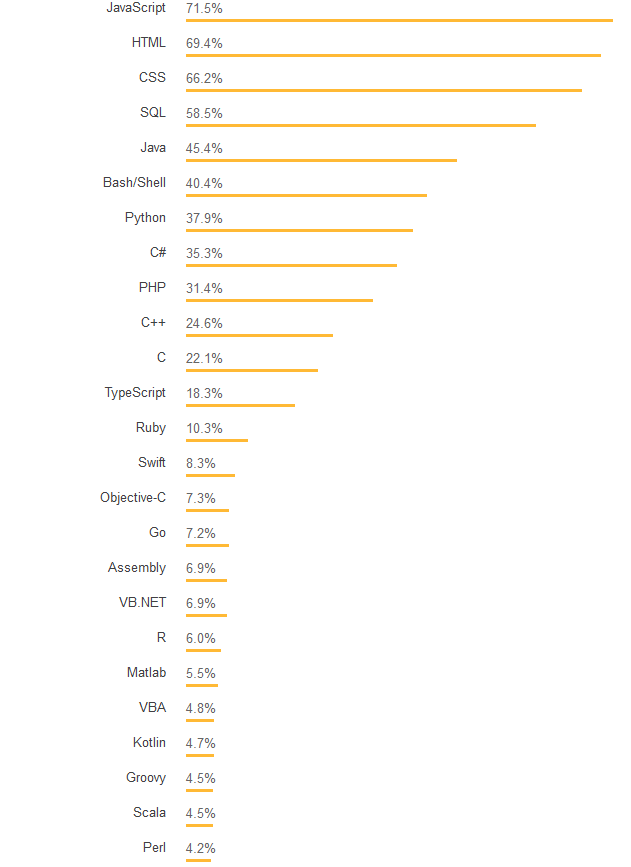
\includegraphics[width=5.00in]{images/tecnologias_populares.png}
\caption{Developer Surver Results 2018. Most popular programming, scripting and markup languagaes technologies.
 Recuperado de: https://insights.stackoverflow.com/survey/2018\#technology-\_-programming-scripting-and-markup-languages}
\label{fig:tecnologias_populares}
\end{figure}

\newpage
Además, el mismo estudio revela que Node.js es la tecnología más popular (con un 49.9\%) dentro del apartado de frameworks, librerías y herramientas:

\begin{figure}[H]
\centering
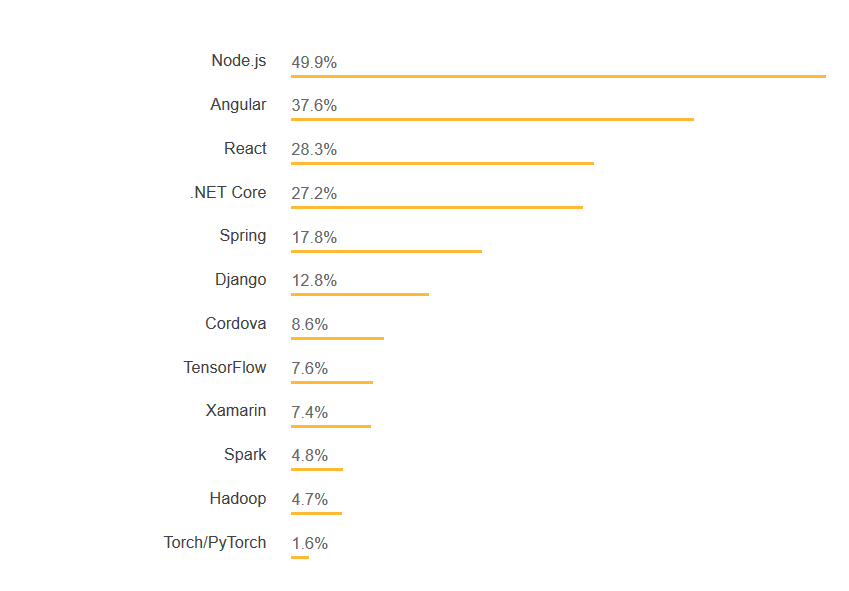
\includegraphics[width=6.00in]{images/frameworks_populares.png}
\caption{Developer Surver Results 2018. Most popular frameworks, libraries and tools. 
Recuperado de: https://insights.stackoverflow.com/survey/2018\#technology-\_-programming-scripting-and-markup-languages}
\label{fig:frameworks_populares}
\end{figure}

\subsection{SQLite}
SQLite es una librería open source que implementa un pequeño gestor de bases de datos SQL. No necesita ejecutarse en un servidor a parte, lee y escribe
directamente de un fichero. Es perfecto para nuestro caso, en el que no se necesitan muchas tablas y éstas no contendran demasiados datos. Todo esto hace
que SQLite se adapte muy bien para sistemas ligeros.
\par
La no necesidad de ejecución en paralelo significa que apenas requiere configuración. Por otro lado, es una librería muy compacta y bastante madura, con 
inicios en el año 2000. Basándonos de nuevo en el \textbf{Developer Survey 2018}, SQLite es el quinto gestor de bases de datos preferido por los desarrolladores,
con un 19.7\%, por delante de gestores muy conocidos como Redis, ElasticSearch, MariaDB u Oracle.
\par
La madurez y popularidad de este gestor hace, como era de esperar, que tenga total compatibilidad con Node.js, y por lo tanto con Express, gracias al módulo
NPM \textbf{sqlite3}.

\subsection{Ionic}
Ionic es un framework open source que nos permite construir aplicaciones híbridas de manera rápida y sencilla. Una aplicación híbrida es, realmente, una
aplicación web que se ejecuta en un WebView dentro del dispositivo, aunque pueden tener acceso directamente a las APIs nativas del dispositivo: GPS, almacenamiento, 
contactos...etc.
\par
La principal ventaja de Ionic es que el mismo desarrollo genera aplicaciones Android, IOS y Web, ya que se trata de aplicaciones web embebidas en un WebView. Además,
Las aplicaciones Ionic están hechas por componentes reutilizables, e Ionic nos ofrece muchísimos componentes (``UI Components``) para construir la interfaz de nuestra
aplicación de manera rápida: botones, alertas, menús, indicadores de carga...etc.
\par
Ionic utiliza tecnologías Web para el desarrollo: TypeScript, HTML y CSS, lo que facilita mucho la migración de una aplicación móvil a una versión web y viceversa: la
mayoría de servicios y lógica puede ser reutilizada, cambiando únicamente los componentes que se utilizan.
\par
Al no tratarse de aplicaciones nativas, Ionic no es indicado para aplicaciones complejas, ya que el rendimiento y la gestión de recursos es mucho menos óptima en
este tipo de aplicaciones. Sin embargo, no es nuestro caso, ya que necesitamos una aplicación sencilla, con una interfaz sencilla que pueda hacer peticiones fácilmente
a una API REST, por lo que Ionic encaja a la perfección.
\par
Además, Ionic ofrece ``live reloading``: no es necesario recompilar o volver a ejecutar nuestra aplicación, si no que los cambios son detectados en caliente y se actualiza
automáticamente.
\lsection{Hub}
Como ya se ha explicado anteriormente, el HUB es la parte central de nuestro sistema. En él reside toda la lógica de negocio, y es el encargado
de comunicarse con la interfaz y los dispositivos.
\subsection{Módulos}
En esta sección se definirán los módulos del HUB y las funciones que cumplen cada uno de ellos. La organización por módulos, además
de permitirnos organizar nuestro software de una manera clara, nos ayuda a construir software flexible: en futuras mejoras del HUB se podrán añadir
nuevos módulos y funcionalidades con facilidad.
\par
Por ejemplo, en el módulo de servicios reside toda la lógica interna, mientras que el módulo enrutador es el encargado de ``traducir`` los datos
provenientes de la red a un modelo de datos conocido e invocar a los diferentes servicios. De esta forma, si en un trabajo futuro queremos añadir
dispositivos bluetooth crearemos un módulo bluetooth que reutilice nuestros servicios.
\par
Otro ejemplo sería la migración de nuestra base de datos a otro motor diferente; sólo necesitaríamos cambiar el módulo repositorio, el resto del sistema
se mantendría intacto.
\par
Cada módulo debe ser independiente del resto, y la modificación interna de un módulo no debería requerir la modificación del resto de módulos.
\subsection{Módulo enrutador}
Este módulo es el encargado de gestionar las conexiones entrantes y de manejar la información proveniente del exterior. Para nuestro caso, que utilizamos
el protocolo HTTPS, en este módulo residirán las implementaciones de las APIS anteriormente definidas. Se encarga de implementar todas las rutas, encapsular
los diferentes parámetros en objetos de nuestro modelo y enviar las respuestas y códigos necesarios tras la invocación al módulo de servicios.
\subsection{Módulo middleware}
A pesar de haber separado este módulo del módulo enrutador, este módulo está totalmente ligado a la utilización del protocolo HTTPS. 
Se trata de un módulo totalmente independiente del módulo enrutador, y tiene dos funciones principales:
\begin{itemize}
\setlength\itemsep{6pt plus 1pt minus 1pt}
\item Interceptar todas las peticiones antes de que lleguen al enrutador y validar las cabeceras y el token JWT. Si el token no es válido entonces
se envía un 401 Unauthorized sin llegar al enrutador.
\item Interceptar los errores que se provoquen durante la ejecución del programa (independientemente del módulo) y traducirlos a respuestas HTTPS. Para esto 
es necesario utilizar un modelo común de error que pueda ser interceptado por este módulo.
\end{itemize}
\subsection{Módulo de servicios}
En este módulo reside la totalidad de nuestra lógica de negocio. A este módulo ya llegan objetos modelados con nuestro modelo de datos, y es totalmente
independiente del protocolo utilizado. Se encarga de hacer llamadas a los repositorios y de aplicar la lógica correspondiente en cada uno de los casos.
\par
Un ejemplo de esta lógica es el registro de dispositivos; una vez recibido un dispositivo y sus correspondientes comandos, el servicio se encarga de hacer
las comprobaciones correspondientes y guardar el dispositivo y después sus comandos.
\par
Además, el módulo de servicios transforma los posibles errores provenientes de los repositorios para encapsularlos en errores internos. Un ejemplo sería
transformar un error \textbf{``14 SQLITE\_CANT\_OPEN``} en el siguiente error: \textbf{``Error 01: no se ha podido acceder a la base de datos sqlite``}.
\par
Tanto la entrada como la salida de datos de los métodos de nuestros servicios seguirán el modelo de datos del HUB.
\subsection{Módulo repositorio}
Este módulo contiene toda la gestión de los datos del HUB. Es invocado por el módulo de servicios, y 
es el encargado de gestionar las conexiones con la base de datos e insertar/obtener datos de la misma.
Este módulo recibe datos modelados con nuestro modelo de datos, pero no necesariamente la manera de enviarlos/guardarlos tiene que coincidir con nuestro modelo 
de datos. Sin embargo, el retorno de los métodos de este módulo sí serán datos modelados.
\par
Si en un futuro se realizasen llamadas a terceros, una API de Google por ejemplo, las llamadas a esas APIS también se realizarían desde este módulo.
\subsection{Vista general}
Por lo tanto, el diseño esquemático de la arquitectura interna del hub es el siguiente:
\begin{figure}[H]
\centering
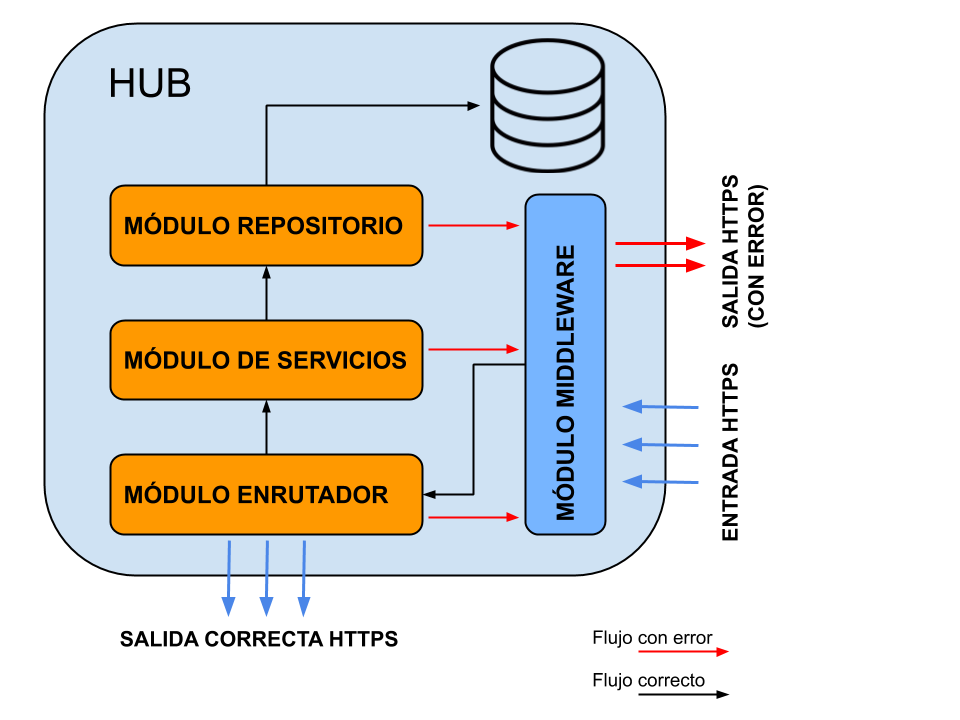
\includegraphics[width=6.00in]{images/arquitectura_hub.png}
\caption{Arquitectura interna del hub}
\label{fig:arquitectura_hub}
\end{figure}
\subsection{Seguridad}
\lsection{Interfaz}
En esta sección se describirán los distintos componentes y pantallas que nuestra aplicación tendrá así como los diferentes servicios. 
\subsection{Pantallas}
Como se ha explicado anteriormente, una de las grandes ventajas de Ionic es la enorme cantidad de UI Components ya hechos que nos ofrece.
En esta sección, se explicarán las pantallas de la aplicación y el flujo entre ellas, y se explicarán los componentes utilizados para cada
una de ellas.
\subsubsection{Diagrama de flujo de las pantallas}
Un diagrama de flujo nos ayuda a entender la navegabilidad de nuestra aplicación. Para evitar sobrecargar el diagrama se han omitido todas
las pantallas que consisten en ``pop-ups`` con diálogos de confirmación, selección, etc. a excepción de la pantalla de confirmación de eliminación del
dispositivo (todas las pantallas de la aplicación pueden verse en el Anexo A del documento).
\par
Para nuestra aplicación, se han diseñado cuatro pantallas principales:
\begin{itemize}
\item\textbf{Pantalla login}: esta pantalla nos permite acceder al sistema. Si los datos introducidos son correctos navegamos automáticamente 
a la pantalla de listado de dispositivos.
\item\textbf{Pantalla listado de dispositivos}: es la pantalla principal de la aplicación. Nos permite visualizar todos los dispositivos y parte
de su información (nombre, información, localización). Nos permite crear nuevas localizaciones, filtrar los dispositivos por localización y eliminar
dispositivos. Se puede volver a la pantalla de login pulsando en el botón de logout, ir a la vista en detalle del dispositivo pulsando sobre un
dispositivo, y navegar a la pantalla de configuración con el menú inferior de navegación.
\item\textbf{Pantalla configuración}: comparte cabebcera y menú inferior de navegación con la pantalla listado de dispositivos. Nos permite, en el
caso de que tengamos permisos, añadir usuarios, modificar nuestro usuario y reestablecer el HUB a su estado de fábrica.
\item\textbf{Pantalla detalle dispositivo}: esta pantalla muestra en detalle la información de un dispositivo. Nos permite eliminarlo, editarlo y
enviarle comandos. Además del nombre, la información y la localización podemos ver la hora última a la que el dispositivo envió información al HUB,
así como su frecuencia de actualización.
\end{itemize}
\begin{figure}[H]
\centering
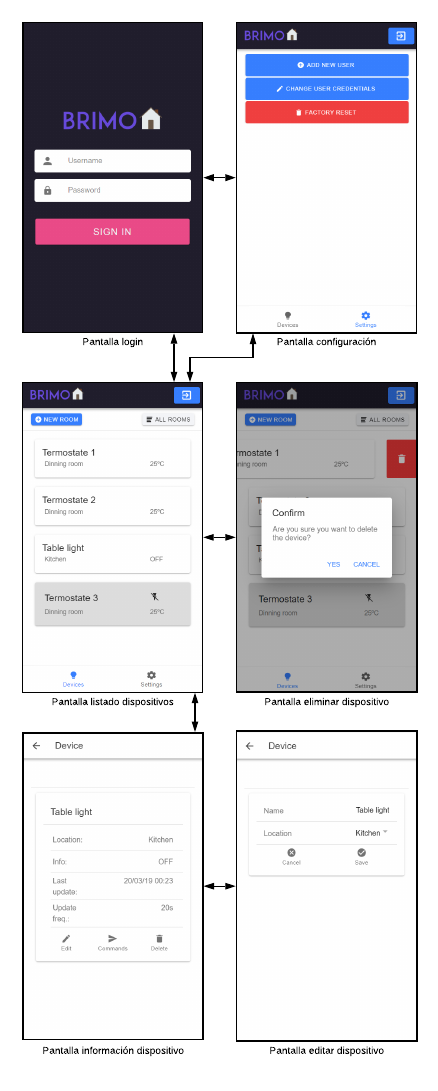
\includegraphics[width=3.50in]{images/flujo_pantallas.png}
\caption{Flujo de pantallas de la interfaz}
\label{fig:flujo_pantallas}
\end{figure}

\subsubsection{Componentes}
Para el desarrollo de la aplicación se han utilizado los siguientes UI Components de Ionic:
\begin{itemize}
\item\textbf{ion-button}: son un componente básico de la UI. Se trata de botones, pueden ser personalizados con iconos, colores, formas...etc.
\item\textbf{ion-icon}: otro componente básico de la UI. Este componente nos permite encapsular iconos en componentes ionic. Ionic ofrece una librería de
iconos bastante extensa, de la cual se han sacado todos los iconos de la aplicación: https://ionicons.com/.
\item\textbf{ion-input}: son inputs encapsulados en componentes ionic. Existen diferentes tipos de inputs: text, password, email, etc. y pueden ser customizados
de diferentes maneras. Se han utilizado, por ejemplo, en la pantalla de login, para introducir usuario y contraseña.
\item\textbf{ion-tabs}: son un componente de navegación. Cada ``tab`` corresponde a una pantalla, y navegar entre ellas a través de la barra inferior de
navegación. En nuestro caso, la aplicación contiene dos tabs: ``devices`` y ``settings``, correspondientes a las pantallas listado de dispositivos y
de configuración.
\item\textbf{ion-header}: nos permite añadir una cabecera a la pantalla. En nuestro caso, la cabecera principal (igual para todas las tabs), contiene un botón
de logout y el logo de la aplicación.
\item\textbf{ion-cards}: se trata de un componente estándar a la hora de hacer interfaces en ionic, y sirven para agrupar información por bloques. En nuestro caso,
 se utilizan cards en las pantallas de listado de dispositivos y de información/edición del dispositivo. En la pantalla de listado de dispositivos
 cada dispositivo corresponde a una ``ion-card``. Tienen subcomponentes como header, title, subtitle, content, etc.
\item\textbf{ion-list}: este componente nos permite hacer listas de otros componentes. En el caso de nuestra aplicación lo usamos en la pantalla de listado
de dispositivos, donde hacemos una lista de ``ion-cards``; y en la pantalla de configuración, donde hacemos una lista de ``ion-buttons``.
\item\textbf{ion-item-sliding}: son componentes deslizables. Se puede customizar de diferentes maneras, y añadir callbacks o componentes ocultos que aparecen
cuando el componente padre se desliza. En nuestro caso, en la pantalla de dispositivos, cada uno de ellos, a parte de ser un ion-card es un item-sliding, lo que
nos permite deslizar el dispositivo a la izquierda para que se muestre el botón de eliminar dispositivo.
\end{itemize}
\newpage
En el siguiente ejemplo se muestran los componentes utilizados en la pantalla de listado de dispositivos:
\begin{figure}[H]
\centering
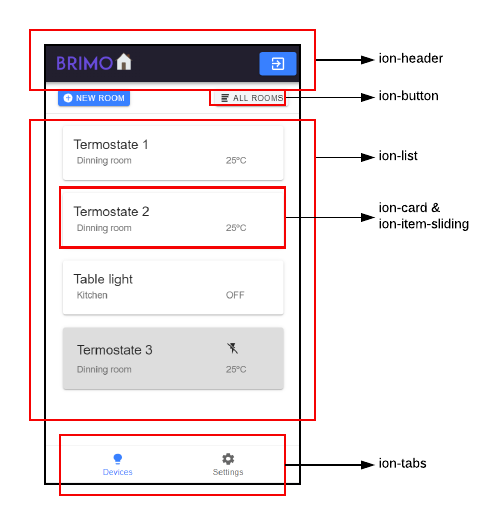
\includegraphics[width=3.50in]{images/ion_components.png}
\caption{Componentes utilizados en la pantalla listado de dispositivos}
\label{fig:ion_components}
\end{figure}

\subsection{Servicios}
Los servicios sirven para compartir funcionalidad entre los componentes. En nuestro caso, serán los encargados de comunicarse con el exterior, es decir, de hacer peticiones al HUB.
Los servicios son independientes de la interfaz, es la interfaz quien los invoca. Por ejemplo, en la pantalla de login, la interfaz se encarga de recoger los datos (usuario y
contraseña) e invocar al servicio de login, que tras hacer una petición al HUB devolverá una respuesta que será procesada de nuevo por la interfaz, mostrando un mensaje de error en
caso de fallo o navegando a la pantalla principal en caso de éxito.
\par
Para el desarrollo de nuestra aplicación hemos creado dos servicios que se encargarán de comunicarse con el HUB y un servicio para comunicar componentes entre sí:
\begin{itemize}
\item\textbf{Servicio de autenticación}: se encarga de comprobar si el usuario está logado y de recuperar el token JWT. Además, este servicio hace las llamadas de login y registrar/modificar
usuario. Cuando se hace una llamada de login el token JWT obtenido se guarda en la memoria del dispositivo, para ser recuperado cada vez que se hace una petición.
\item\textbf{Servicio de comunicación}: se encarga de comunicarse directamente con el HUB. Utiliza el servicio de autenticación para recuperar el token JWT y añadirlo en las cabeceras de 
cada petición. Este servicio sirve para añadir habitaciones, eliminar dispositivos, editar dispositivos...etc.
\item\textbf{Servicio compartido}: este servicio se encarga de comunicar componentes entre sí. Funciona con observables, a los que cada componente se suscribe en el caso de ser necesario.
Funciona, por ejemplo, para saber que el token ha caducado: si cualquier petición recibe un 401 entonces envía un evento a este servicio para que el resto de componentes (que se haya suscrito
a dicho tipo de eventos) lo sepa y la aplicación redirija automáticamente a la pantalla de login.
\end{itemize}

